% ============================================================
% Question Bank: ch03-03 Subtracting Integers
% Topic Title: Subtracting Integers
% CCSS: 7.NS.A.1
% Questions: 27 (15 MC + 6 SA + 6 Graphical)
% ============================================================

% --- Multiple Choice Questions (15) ---

\begin{practiceQuestion}{3-3-q01}{mc}
\begin{questionText}
What is $5 - 13$?
\end{questionText}
\choiceA{$8$}
\choiceB{$-8$}
\choiceC{$18$}
\choiceD{$-18$}
\correctAnswer{B}
\explanation{Rewrite as adding the opposite: $5 + (-13) = -8$. The larger absolute value ($13$) is negative, so the result is $-8$.}
\end{practiceQuestion}

\begin{practiceQuestion}{3-3-q02}{mc}
\begin{questionText}
What is $(-6) - (-14)$?
\end{questionText}
\choiceA{$-20$}
\choiceB{$20$}
\choiceC{$-8$}
\choiceD{$8$}
\correctAnswer{D}
\explanation{Subtracting a negative means adding: $(-6) + 14 = 8$. Different signs: $14 - 6 = 8$, positive.}
\end{practiceQuestion}

\begin{practiceQuestion}{3-3-q03}{mc}
\begin{questionText}
Which expression is equivalent to $9 - (-5)$?
\end{questionText}
\choiceA{$9 - 5$}
\choiceB{$9 + 5$}
\choiceC{$-9 + 5$}
\choiceD{$-9 - 5$}
\correctAnswer{B}
\explanation{Subtracting a negative is the same as adding: $9 - (-5) = 9 + 5 = 14$.}
\end{practiceQuestion}

\begin{practiceQuestion}{3-3-q04}{mc}
\begin{questionText}
The high temperature on Monday was $8°$F. The low temperature was $-11°$F. What was the difference between the high and low temperatures?
\end{questionText}
\choiceA{$3°$F}
\choiceB{$-3°$F}
\choiceC{$19°$F}
\choiceD{$-19°$F}
\correctAnswer{C}
\explanation{Difference: $8 - (-11) = 8 + 11 = 19°$F. Subtracting a negative adds the values.}
\end{practiceQuestion}

\begin{practiceQuestion}{3-3-q05}{mc}
\begin{questionText}
What is $(-10) - 7$?
\end{questionText}
\choiceA{$3$}
\choiceB{$-3$}
\choiceC{$17$}
\choiceD{$-17$}
\correctAnswer{D}
\explanation{Rewrite: $(-10) + (-7) = -17$. Same signs: add $10 + 7 = 17$, keep negative.}
\end{practiceQuestion}

\begin{practiceQuestion}{3-3-q06}{mc}
\begin{questionText}
A student says $(-8) - (-3) = -11$. What is the student's mistake?
\end{questionText}
\choiceA{The student added instead of subtracting}
\choiceB{The student forgot to flip the sign of $-3$ to $+3$}
\choiceC{The student multiplied instead of subtracting}
\choiceD{There is no mistake; $-11$ is correct}
\correctAnswer{B}
\explanation{When subtracting a negative, change to addition: $(-8) - (-3) = (-8) + 3 = -5$. The student kept $-3$ instead of flipping it to $+3$.}
\end{practiceQuestion}

\begin{practiceQuestion}{3-3-q07}{mc}
\begin{questionText}
What is $0 - (-11)$?
\end{questionText}
\choiceA{$-11$}
\choiceB{$0$}
\choiceC{$11$}
\choiceD{$-22$}
\correctAnswer{C}
\explanation{$0 - (-11) = 0 + 11 = 11$. Subtracting a negative is adding.}
\end{practiceQuestion}

\begin{practiceQuestion}{3-3-q08}{mc}
\begin{questionText}
The temperature dropped from $12°$C to $-4°$C. What was the change in temperature?
\end{questionText}
\choiceA{$8°$C}
\choiceB{$-8°$C}
\choiceC{$16°$C}
\choiceD{$-16°$C}
\correctAnswer{D}
\explanation{Change $=$ new $-$ old $= -4 - 12 = -4 + (-12) = -16°$C. The temperature decreased $16$ degrees.}
\end{practiceQuestion}

\begin{practiceQuestion}{3-3-q09}{mc}
\begin{questionText}
What is $(-9) - (-9)$?
\end{questionText}
\choiceA{$-18$}
\choiceB{$18$}
\choiceC{$0$}
\choiceD{$-9$}
\correctAnswer{C}
\explanation{Any number minus itself equals $0$: $(-9) - (-9) = (-9) + 9 = 0$.}
\end{practiceQuestion}

\begin{practiceQuestion}{3-3-q10}{mc}
\begin{questionText}
Which subtraction problem has the greatest result?
\end{questionText}
\choiceA{$(-2) - 8$}
\choiceB{$4 - (-6)$}
\choiceC{$(-5) - (-1)$}
\choiceD{$1 - 9$}
\correctAnswer{B}
\explanation{A: $-10$. B: $4 + 6 = 10$. C: $(-5) + 1 = -4$. D: $-8$. The greatest result is $10$.}
\end{practiceQuestion}

\begin{practiceQuestion}{3-3-q11}{mc}
\begin{questionText}
A helicopter is at $2{,}400$ feet. A submarine is at $-600$ feet. What is the vertical distance between them?
\end{questionText}
\choiceA{$1{,}800$ feet}
\choiceB{$2{,}000$ feet}
\choiceC{$3{,}000$ feet}
\choiceD{$3{,}600$ feet}
\correctAnswer{C}
\explanation{Distance: $|2{,}400 - (-600)| = |2{,}400 + 600| = |3{,}000| = 3{,}000$ feet.}
\end{practiceQuestion}

\begin{practiceQuestion}{3-3-q12}{mc}
\begin{questionText}
What is $(-2) - 4 - (-9)$?
\end{questionText}
\choiceA{$-15$}
\choiceB{$3$}
\choiceC{$-3$}
\choiceD{$15$}
\correctAnswer{B}
\explanation{Rewrite: $(-2) + (-4) + 9$. Negatives: $-2 + (-4) = -6$. Then $-6 + 9 = 3$.}
\end{practiceQuestion}

\begin{practiceQuestion}{3-3-q13}{mc}
\begin{questionText}
If $a = -5$ and $b = -12$, what is $a - b$?
\end{questionText}
\choiceA{$7$}
\choiceB{$-7$}
\choiceC{$17$}
\choiceD{$-17$}
\correctAnswer{A}
\explanation{$a - b = (-5) - (-12) = (-5) + 12 = 7$.}
\end{practiceQuestion}

\begin{practiceQuestion}{3-3-q14}{mc}
\begin{questionText}
The Dead Sea surface is at $-1{,}412$ feet. A city nearby is at $2{,}575$ feet elevation. What is the difference in elevation?
\end{questionText}
\choiceA{$1{,}163$ feet}
\choiceB{$-1{,}163$ feet}
\choiceC{$3{,}987$ feet}
\choiceD{$-3{,}987$ feet}
\correctAnswer{C}
\explanation{$2{,}575 - (-1{,}412) = 2{,}575 + 1{,}412 = 3{,}987$ feet.}
\end{practiceQuestion}

\begin{practiceQuestion}{3-3-q15}{mc}
\begin{questionText}
Which expression gives a negative result?
\end{questionText}
\choiceA{$(-3) - (-10)$}
\choiceB{$5 - (-2)$}
\choiceC{$(-1) - (-1)$}
\choiceD{$2 - 11$}
\correctAnswer{D}
\explanation{A: $(-3) + 10 = 7$. B: $5 + 2 = 7$. C: $(-1) + 1 = 0$. D: $2 + (-11) = -9$. Only D is negative.}
\end{practiceQuestion}

% --- Short Answer Questions (6) ---

\begin{practiceQuestion}{3-3-q16}{sa}
\begin{questionText}
What is $(-18) - (-25)$?
\end{questionText}
\correctAnswer{$7$}
\explanation{Rewrite as adding the opposite: $(-18) + 25 = 7$. Different signs: $25 - 18 = 7$, positive.}
\end{practiceQuestion}

\begin{practiceQuestion}{3-3-q17}{sa}
\begin{questionText}
The freezer temperature is $-8°$C. The refrigerator is at $4°$C. How much warmer is the refrigerator than the freezer?
\end{questionText}
\correctAnswer{$12°$C}
\explanation{Subtract: $4 - (-8) = 4 + 8 = 12°$C warmer.}
\end{practiceQuestion}

\begin{practiceQuestion}{3-3-q18}{sa}
\begin{questionText}
Find the distance between $-7$ and $-15$ on a number line.
\end{questionText}
\correctAnswer{$8$ units}
\explanation{Distance $= |{-7} - (-15)| = |{-7} + 15| = |8| = 8$ units.}
\end{practiceQuestion}

\begin{practiceQuestion}{3-3-q19}{sa}
\begin{questionText}
What is $6 - 15 - (-4)$?
\end{questionText}
\correctAnswer{$-5$}
\explanation{Rewrite: $6 + (-15) + 4$. Positives: $6 + 4 = 10$. Negatives: $-15$. Sum: $10 + (-15) = -5$.}
\end{practiceQuestion}

\begin{practiceQuestion}{3-3-q20}{sa}
\begin{questionText}
Mt. Everest's summit is $29{,}032$ feet above sea level. The Mariana Trench is $-36{,}201$ feet. What is the total vertical distance between them?
\end{questionText}
\correctAnswer{$65{,}233$ feet}
\explanation{$29{,}032 - (-36{,}201) = 29{,}032 + 36{,}201 = 65{,}233$ feet.}
\end{practiceQuestion}

\begin{practiceQuestion}{3-3-q21}{sa}
\begin{questionText}
What is $(-30) - 17$?
\end{questionText}
\correctAnswer{$-47$}
\explanation{Rewrite: $(-30) + (-17) = -47$. Same signs: $30 + 17 = 47$, keep negative.}
\end{practiceQuestion}

% --- Graphical Questions (3 GMC + 3 GSA) ---

\begin{practiceQuestion}{3-3-q22}{gmc}
\begin{questionText}
The number line below shows a subtraction problem modeled with arrows. What subtraction problem is shown?

\begin{center}
\begin{tikzpicture}
  \draw[thick,->] (-4.5,0) -- (10.5,0);
  \foreach \x in {-4,...,10} \draw (\x,0.1) -- (\x,-0.1) node[below,font=\small] {$\x$};
  \fill[funBlue] (2,0) circle (0.1);
  \draw[thick,->,funGreen] (2,0.35) -- (8,0.35);
  \node[above,font=\small] at (5,0.4) {$+6$};
  \node[above left,font=\small] at (2,0.1) {start};
\end{tikzpicture}
\end{center}
\end{questionText}
\choiceA{$2 - 6 = -4$}
\choiceB{$2 - (-6) = 8$}
\choiceC{$8 - 6 = 2$}
\choiceD{$8 - 2 = 6$}
\correctAnswer{B}
\explanation{Starting at $2$ and moving $6$ units to the right means adding $6$: $2 + 6 = 8$. This is equivalent to $2 - (-6) = 8$.}
\end{practiceQuestion}

\begin{practiceQuestion}{3-3-q23}{gmc}
\begin{questionText}
The diagram shows two depths in a lake. What is the difference in depth between the dock and the bottom?

\begin{center}
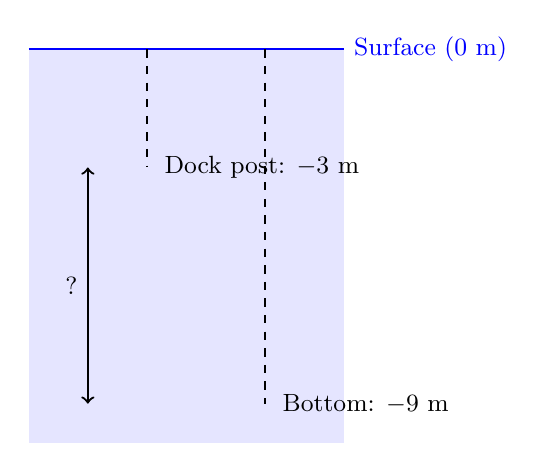
\begin{tikzpicture}[scale=0.5]
  \fill[blue!10] (-1,-10) rectangle (7,0);
  \draw[thick,blue] (-1,0) -- (7,0) node[right,font=\small]{Surface ($0$ m)};
  \draw[thick,dashed] (2,0) -- (2,-3);
  \node[right,font=\small] at (2.2,-3) {Dock post: $-3$ m};
  \draw[thick,dashed] (5,0) -- (5,-9);
  \node[right,font=\small] at (5.2,-9) {Bottom: $-9$ m};
  \draw[thick,<->] (0.5,-3) -- (0.5,-9) node[midway,left,font=\small] {?};
\end{tikzpicture}
\end{center}
\end{questionText}
\choiceA{$3$ meters}
\choiceB{$-6$ meters}
\choiceC{$6$ meters}
\choiceD{$12$ meters}
\correctAnswer{C}
\explanation{Distance $= |{-3} - (-9)| = |{-3} + 9| = |6| = 6$ meters. The bottom is $6$ meters deeper than the dock.}
\end{practiceQuestion}

\begin{practiceQuestion}{3-3-q24}{gmc}
\begin{questionText}
The table shows daily temperature changes for a week. On which day did the temperature drop the most from the previous day?

\begin{center}
\begin{tabular}{|l|c|}
\hline
\textbf{Day} & \textbf{Temp (°C)} \\
\hline
Monday & $5$ \\ \hline
Tuesday & $-1$ \\ \hline
Wednesday & $-4$ \\ \hline
Thursday & $2$ \\ \hline
Friday & $-7$ \\ \hline
\end{tabular}
\end{center}
\end{questionText}
\choiceA{Tuesday}
\choiceB{Wednesday}
\choiceC{Thursday}
\choiceD{Friday}
\correctAnswer{D}
\explanation{Changes: Tue: $-1 - 5 = -6$. Wed: $-4 - (-1) = -3$. Thu: $2 - (-4) = +6$. Fri: $-7 - 2 = -9$. The largest drop is $-9$ on Friday.}
\end{practiceQuestion}

\begin{practiceQuestion}{3-3-q25}{gsa}
\begin{questionText}
The number line shows two points. What is $A - B$?

\begin{center}
\begin{tikzpicture}
  \draw[thick,->] (-8.5,0) -- (4.5,0);
  \foreach \x in {-8,...,4} \draw (\x,0.1) -- (\x,-0.1) node[below,font=\small] {$\x$};
  \fill[funBlue] (-6,0) circle (0.12) node[above=4pt,font=\small] {A};
  \fill[funRed] (3,0) circle (0.12) node[above=4pt,font=\small] {B};
\end{tikzpicture}
\end{center}
\end{questionText}
\correctAnswer{$-9$}
\explanation{$A - B = (-6) - 3 = (-6) + (-3) = -9$.}
\end{practiceQuestion}

\begin{practiceQuestion}{3-3-q26}{gsa}
\begin{questionText}
A mountain peak is at $3{,}200$ feet and a canyon floor is at $-800$ feet, as shown below. What is the elevation difference?

\begin{center}
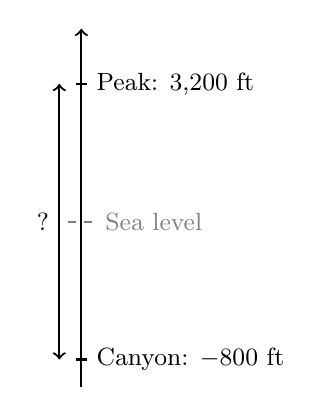
\begin{tikzpicture}[scale=0.35]
  \draw[thick,->] (0,-3) -- (0,10);
  \node[right,font=\small] at (0.2,8) {Peak: $3{,}200$ ft};
  \node[right,font=\small] at (0.2,-2) {Canyon: $-800$ ft};
  \draw[thick] (-0.2,8) -- (0.2,8);
  \draw[thick] (-0.2,-2) -- (0.2,-2);
  \draw[thick,dashed,gray] (-0.5,3) -- (0.5,3) node[right,font=\small] {Sea level};
  \draw[thick,<->] (-0.8,-2) -- (-0.8,8) node[midway,left,font=\small] {?};
\end{tikzpicture}
\end{center}
\end{questionText}
\correctAnswer{$4{,}000$ feet}
\explanation{$3{,}200 - (-800) = 3{,}200 + 800 = 4{,}000$ feet.}
\end{practiceQuestion}

\begin{practiceQuestion}{3-3-q27}{gsa}
\begin{questionText}
The table shows a company's profit and loss each quarter. What is the total profit or loss for the year?

\begin{center}
\begin{tabular}{|l|c|}
\hline
\textbf{Quarter} & \textbf{Result} \\
\hline
Q1 & $-\$4{,}500$ \\ \hline
Q2 & $+\$7{,}200$ \\ \hline
Q3 & $-\$1{,}800$ \\ \hline
Q4 & $+\$3{,}600$ \\ \hline
\end{tabular}
\end{center}
\end{questionText}
\correctAnswer{$\$4{,}500$}
\explanation{Add all values: $(-4{,}500) + 7{,}200 + (-1{,}800) + 3{,}600$. Positives: $7{,}200 + 3{,}600 = 10{,}800$. Negatives: $-4{,}500 + (-1{,}800) = -6{,}300$. Total: $10{,}800 + (-6{,}300) = \$4{,}500$ profit.}
\end{practiceQuestion}
